\documentclass[12pt, letterpaper]{article}

\usepackage{tikz}

\title{musings}
\author{Anna Fritz}
\date{\today}

\begin{document}

\maketitle
\section{Selection Policy}

Prior to this, we assumed that an appraiser would apply their selection policy to generate the best term for attestation. However, in our first attempt at negotiation, the selection policy was hollow and insignificant. It was simply applied as a proof of concept. However, now we consider ways to order protocols such that the selection policy may arrive at tehe ``best'' protocol for attestation. 

\subsection{Refinement trees}

One way to enforce an ordering over protocols may be with a refinement tree. Let us assume that entity A would like to meas T. The request may appear as \emph{R = {meas T}}. Upon receiving the request, the target would enforce their privacy policy 

\begin{figure}

\usetikzlibrary{trees}

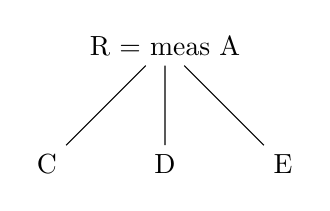
\begin{tikzpicture}
    \node {R = meas A}
        child {node {C}}
        child {node {D}}
        child {node {E}
        };
\end{tikzpicture}  


\end{figure}

\subsection {Possible helpful resources}

In order to arrange protocols with some ordering, we must analyze them. Mitre has written many papers on the topic. 


\begin{itemize}
    \item CPSA 
    \begin{itemize}
        \item Cryptographic Protocol Shapes Analyzer (CPSA) automatically characterizes the possible executions of a protocols
        \item Give the tool a set of assumptions and it will find all outputs 
        \item This tool aims to completely characterize how the protocol could be executed
        \item In this case, a protocol is an exchange of messages. In our case, there won't be an exchange of messages, just the messages themselves that need some sort of ordering.
        \item Realized skeleton is the abstracted away details of the protocol analysis

        \item Useful things I think they define: 
        \begin{itemize}
            \item event = message transmission or reception 
            \item outbound message
            \item distinction between node space and protocol space where the node space includes a map to set of traces 
        \end{itemize}
        
        \item \textbf{What I'm thinking...} This tool creates trees that depict all possible protocol executions. We don't care so much about the interactions between communicating peers so much as the possible measurement operations. I think the mathematical properties and definitions here are useful. But we really need to focus more on protocols and less on the communication between target and appraiser. 


        \item To get it working is a pain...  issues with cabal and versioning. Finally got it working so that you could call ** get cabal working to use tool

        getting this error message 
        
        Warning: could not create symlinks in /Users/annarosefritz/.cabal/bin for
        cpsa, cpsagraph, cpsashapes, cpsaannotations, cpsadiff, cpsasas, cpsaprot,
        cpsapp, cpsajson, cpsadebase, cpsamatch, cpsainit, cpsagoalsat, cpsa2latex
        because the files exist there already and are not managed by cabal. You can
        create symlinks for these executables manually if you wish. The executable
        files have been installed at /Users/annarosefritz/.cabal/bin/cpsa, 
    \end{itemize}
    \item Skeletons, Homomorphisms, and Shapes/ Characterizing Protocol Executions
    \begin{itemize}
        \item When looking to analyze protocols, one starts with an initial set, a singleton set. 
        \item The author's use a homomorphism to map nodes of one peer $A_0$ to another $A_1$. This is useful as $A_1$ may provide additional details about $A_0$.
        \item They also introduce a \textbf{skeleton} which consists of a finite set of nodes, a partial order over the nodes where the order reflects precedence, key, and atomic values.   
    \end{itemize}
\end{itemize}






\end{document}